\chapter{Joint Decisions}
\label{ch:jointtrips}
% ##################################################################################################################

\hfill \textbf{Author:} Thibaut Dubernet

\begin{center} 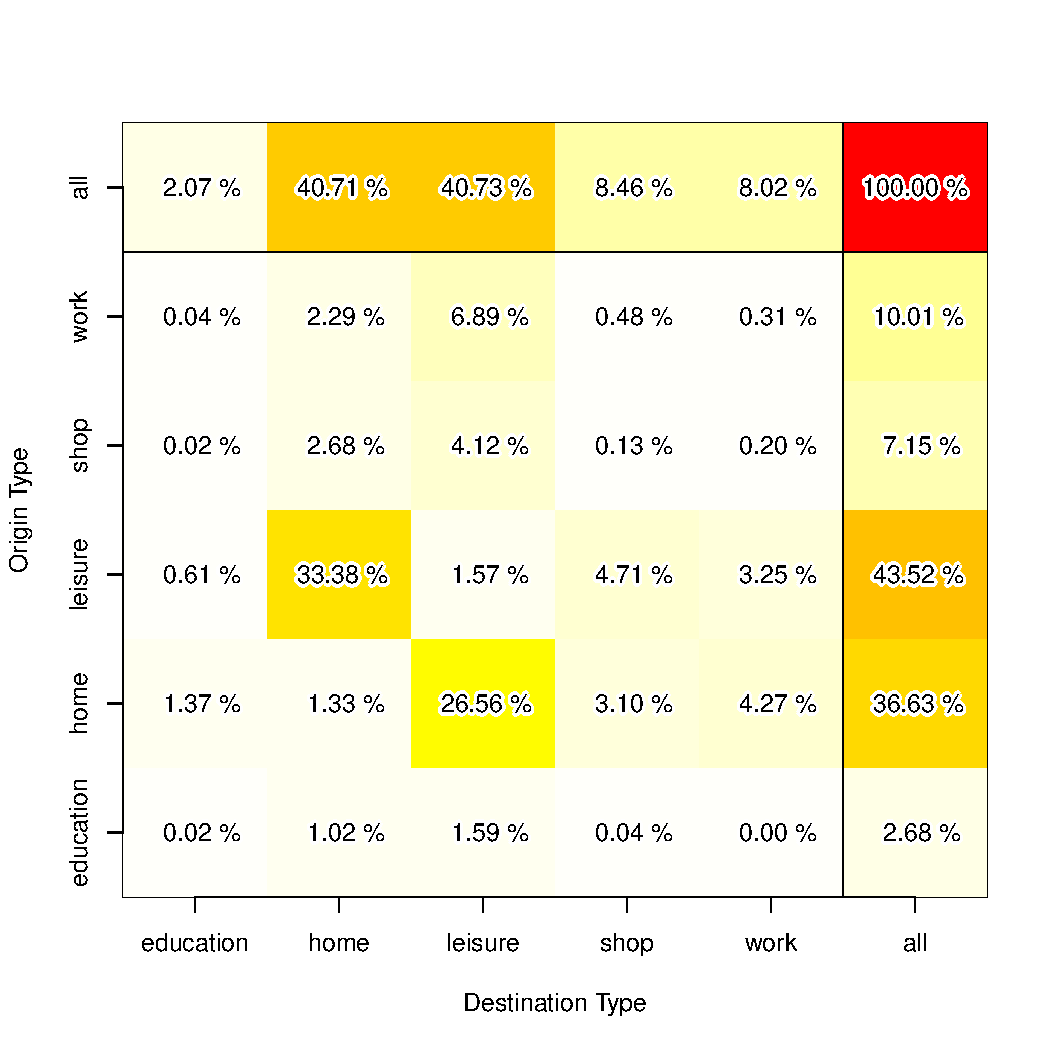
\includegraphics[width=0.4\textwidth, angle=0]{extending/figures/Jointtrips/passenger-per-type-ju3-asShareOfPassengerTrips} \end{center}

\editdone{This text has undergone the professional edit. Please no grammatical changes anymore! They are most-probably wrong.}

\createStandardInformation{todo}{todo}{todo}{\citet{DubernetAxhausen_TransLett_2013}}

% ##################################################################################################################
{ % scope for chapter commands: 
% Figures
\newcommand\insfig[2]{%
	\insfigwidth{#1}{#2}{.8\textwidth}
}
\newcommand\insfigwidth[3]{%
\createfigure{#1}{#1}{}{%
		\includegraphics[width=#3]{extending/figures/Jointtrips/#2}%
		}{}%
}

\newcommand\inssubfigwidth[3]{%
\createsubfigure{#2}{%
		\includegraphics[width=#1]{extending/figures/Jointtrips/#3}%
		}{}{\quad}%
}
\newcommand\inssubfig[2]{%
\inssubfigwidth{.46\textwidth}{#1}{#2}%
}
\newcommand\insfigwithsubfigs[2]{%
\createfigure{#1}{#1}{}{%
		#2%
		}{}%
}

% ##################################################################################################################
This chapter describes the extension of \gls{matsim} to consider what we call \emph{joint decisions}. Section~\ref{sec:td:intro} explains what we call a joint decision, and gives an overview of why such processes
are important in transportation. Section~\ref{sec:td:algo} then presents concepts to model this behavior, a generalization of the \gls{matsim} algorithm to search for solutions to the \emph{joint planning problem}, and gives technical insights on how this implementation could be achieved, given the MATSim software architecture.

% ##################################################################################################################
\section{Joint Decisions and Transport Systems}
\label{sec:td:intro}
% ============================================================================
\subsection{Motivation}
In recent years, there has been a growing interest in the social dimension of travel and how travel decisions are influenced, not only by the global state of the transportation system, but also by joint decisions and interactions with social contacts.

A very active field of research is the study and modeling of intra-household interactions and joint decision-making, often using the classical random utility framework extended to group decision-making. Examples of household scheduling models include: \citet{ZhangEtAl_TransResB_2005, ZhangJEtAl_TRR_2007, KatoMatsumoto_TransResB_2009, BradleyVovsha_Transportation_2005, GliebeKoppelman_Transportation_2005,
GliebeKoppelman_Transportation_2002, HoCAndMulley_Transportation_2013, VovshaGupta_Transportation_2013}. Most of those models are specific to given household structures; in particular, separate models need to be estimated for different household sizes.

Another class of approaches, more oriented toward multi-agent simulation than analysis, is the use of optimization algorithms to generate households plans. These algorithms handle the household scheduling problem by transforming it into a deterministic utility maximization problem. Contrary to the previously presented approaches, those alternatives do not lead to the estimation of a model against data. Examples of approaches rooted in operations research include: \citet{Recker_TRR_1995}, for which \citet{ChowRecker_TranResB_2012} designed a calibration method, or \citet{GanRecker_TransResB_2008}. Another attempt to generate plans for households uses a genetic algorithm, building on a previous genetic algorithm for individual plan generation \citep{CharyparNagel2005ga4acts, MeisterEtAl_Transportation_2005}, using a joint utility. Finally, \citet{LiaoFEtAl_Transportation_2013} formulate the problem of creating schedules for two persons traveling together as finding the shortest path in a ``supernetwork'', but note that their model is specific to the two person problem and that extension to larger numbers of agents may prove to be computationally expensive. All those approaches remained experimental, and were not integrated into multi-agent simulation tools.

Another class of methods aiming at multi-agent simulations is constituted rule based systems, which use heuristic rules to construct household plans, such as \citet{MillerEtAl_Transportation_2005, ArentzeTimmermans_TransResB_2009}.

Other authors have investigated the role of more general social networks on travel. One of the main incentives to conduct such studies comes from the continuous increase of the share of leisure purpose trips  \citep{SchlichEtAl_TransportRev_2004,Axhausen_DonaghyEtAl_2005}. This trend represents a challenge for travel behavior modeling, as those trips are much more difficult to forecast than commuting trips; they are performed more sporadically and data from such trips is much more difficult to collect---particularly concerning location and event attributes, necessary to make models that are more than just random noise. A better understanding of how leisure trip destination choices are made is essential to improve the accuracy of those forecasts.

Various studies have been conducted to confirm that making social contacts is an important factor in leisure trip destination choice, or activity duration choice. Examples of empirical work include: \citet{CarrascoJAHabib_IATBR_2009}; \citet{HabibCarrascoJA_TRR_2011} or \citet{MooreJEtAl_Transportation_2013}. All these studies show strong influence of social contacts on the spatial and temporal distribution of activities. In a simulation experiment, \citet{Frei_PhDThesis_2012} demonstrated that considering social interactions in leisure location choice helps increase the accuracy of predicted leisure trip distance distribution.

Another field of empirical research studies the spatial characteristics of social networks. For instance, \citet{CarrascoJAEtAl_TRR_2008} studied the relationship between individual's socioeconomic
characteristics and the spatial distribution of their social contacts. This kind of empirical work allows specification and estimation of models able to generate synthetic social networks, given sociodemographic attributes and home location. An example of such a model, based on the results of a survey in Switzerland, can be found in \citet{ArentzeEtAl_TRB_2012}. This kind of model is essential if one wants to include social network interactions in microsimulation model.

This integration of social networks in multi-agent simulation frameworks has already been attempted by other authors. Due to their disaggregated description of the world, such models are particularly well-suited to complex social topologies representation. \citet{HanQEtAl_TransResPartA_2011} present experiments using social networks to guide activity location choice set formation in the \gls{feathers} multi-agent simulation framework. Using a simple scenario with 6\,agents forming a \emph{clique}, %(a network where all agents have social ties with all other agents),
they consider the influence of various processes like information exchange and adaptation to the behavior of social contacts to increase the probability of an encounter. They do not, however, represent \emph{joint decisions}, such as the scheduling of a joint activity. The same kind of processes have been investigated by \citet{Hackney_PhDThesis_2009}, using more complex network topologies (within the MATSim framework) used in this paper. \citet{RonaldEtAl_TransResB_2012, MaEtAl_TRR_2011, MaEtAl_IATBR_2012} present agent based systems, which integrate joint decision-making mechanisms, based on rule based simulations of a bargaining processes. They are not yet integrated into any operational mobility simulation platform.

Those remarks point the need to include explicit coordination in multi-agent simulation platforms.

% ============================================================================
\subsection{The Joint Planning Problem}
%---------------------------------------------------------------------------
Here, we present a simulation framework able to represent \emph{joint decisions}: that is, behavior requiring \emph{explicit} coordination between individuals---such as shared rides, social activities or intra-household task allocation. The basic idea is that social contacts will make such a joint decision if it results in an improvement in the satisfaction of all participants. Modeling the interaction of individuals with possibly conflicting objectives has been the subject of game theory for decades, making this theoretical framework particularly well suited for the problem at hand.

Interestingly, game theoretic view of transportation systems has been popular since the seminal work of \citet{Wardrop_PICE_1952}. The essential underlying concept is a view of the transportation system as a set of shared resources (road space, public transport vehicle seats\ldots), for which individuals compete; individuals in the population try to maximize their own satisfaction, given the resources left available by others. Game theory studies \emph{solution concepts} for such strategic interactions. A game theoretic solution concept is a definition of which states are \emph{equilibria}: that is, \emph{stable} under assumption of rationality---a state is considered stable if no agent/player has an incentive to change its behavior. The static, trip-based approach of \citet{Wardrop_PICE_1952} has been refined and extended with time. In particular, the equilibrium idea can be quite readily transferred to the \emph{activity based} framework: individuals try not only to optimize their trips, but their whole day. This is, in particular, the approach of \gls{matsim} \citep{Axhausen_SSRL_2006, NagelFloetteroed2009IatbrResourceInBook}.

Most solution concepts in transportation are akin to the Nash equilibrium: a state where no individual can improve its satisfaction by \emph{unilaterally} changing its behavior. This kind of solution concept does not allow to represent joint decisions. This can be illustrated by a classical game, called the \emph{House Allocation Problem} \citep{SchummerVohra_NisanEtAl_2007}. This game consists of $n$ players and $n$ houses. Moreover, each player has its individual ordering of the houses, from the most preferred to the least preferred, and players prefer being allocated alone to any house rather than to a house occupied by someone else. The strategy of a player centers around the house where the player chooses to live.

An interesting feature of this game is that any one-to-one allocation of players to houses is a Nash Equilibrium; no player can improve its payoff by \emph{unilaterally} changing its strategy, as it would require choosing an occupied house. This result, however, contradicts basic intuition about the stability of such an allocation. In this particular case, a more realistic solution concept is the \emph{Absence of Blocking Coalition}; given a one-to-one allocation of houses to players, a blocking coalition is a set of players which could all be better off by reallocating their houses among themselves. It should be noted that both solution concepts correspond to rational agents, \ie agents having a preference ordering over outcomes. The only difference lies in the degree of communication allowed.

In the activity-based framework, this solution concept naturally becomes what we define as the \emph{Absence of Improving Coalition} solution concept. An improving coalition for a given allocation of daily plans is a set of social contacts who can all feel themselves to be better off by \emph{simultaneously} changing their daily plan---for instance, by switching from separate dinners at home to a joint dinner at a restaurant.
The simulation of joint decision consists of searching an allocation of daily plans without such coalitions.

% ##################################################################################################################
\section{An Solution Algorithm for the Joint Planning Problem: a Generalization of the MATSim Process}
\label{sec:td:algo}
% ============================================================================
\subsection{Algorithm}
Given this theoretical framework, one needs to design and implement an algorithm to search for allocations of daily plans to individuals that satisfy this solution concept. This implementation consists of two groups of components:
%
\begin{enumerate}
\item a \lstinline|Controler| that implements the extension of the \gls{matsim} co-evolutionary algorithm, outlined hereafter. It is implemented in a modular fashion, to be easily adapted to the specific need of different simulation scenarios and
\item specific implementations of the modular components, namely replanning strategies and scoring functions, to allow explore the set of possible \emph{joint plans} and representations of possible preferences specific to joint decisions.
\end{enumerate}

\paragraph{Controler}

The \gls{matsim} framework provides a \lstinline|Controler| to build and configure co-evolutionary algorithms, where agents each optimize their plan given the (evolving) state of the transport system.

Unfortunately, this approach makes choices of agents independent---which, of course, goes against the simulation of \emph{joint decisions}. To implement an algorithm searching for states without
blocking coalitions, one needs a way to represent the influence of explicit coordination on daily plan utility. This is solved by including \emph{joint plans} constraints. A joint plan is a set of
individual plans executed simultaneously. Different copies of the same individual plan can be part of different joint plans---for instance, an agent might go to a given restaurant alone, with members of its
household or with a group of friends. The score of the different copies will take into account the influence of the joint plan to which it pertains. Those joint plan constraints are included using heuristic
rules, applied after mutation operators are applied, and are classified as strong or weak constraints---weak constraints are considered when selecting plans for execution, but are allowed to be broken when merely selecting plans for mutation. They are then part of the evolution process. In the current application, the heuristic rules consist of joining newly created plans with joint trips (strong), or with leisure activities at the same location at the same time (weak).

To allow handling joint plans, replanning needs to be performed for groups of agents. This is straightforward for households; all agents of the same household are always handled as a single group. For more general social networks, agents are handled with all agents with whom they have a joint plan, plus some social contacts with whom new joint plans can be created.

For each group, two actions are then possible. For most groups, an allocation of existing plans---fulfilling the joint plans constraints---is selected for execution. Based on plan scores, randomized by adding an extreme value distributed error term, an algorithm inspired by the ``Top Trading Cycle'' algorithm used for the ``House Allocation Problem'' \citep{SchummerVohra_NisanEtAl_2007} searches for an allocation without improving coalitions.

For the other groups, a plan allocation is selected and copied. The copied plans then undertake mutation, to make the agents explore new alternative joint plans. Which mutation is performed  determines which alternative plans will be tried out by the agent.

Agents have a limited memory size, keeping by default at most 3\,plans per joint plan composition, and 10\,plans in total. If this limit is exceeded, one should keep the plans which have the highest probability of creating improving coalition: that is, preferable to the other plans in the agent's memory. To this end, a lexicographic ordering is used; the process removes the joint plan  maximizing the number of individual plans which are the worst of the agents' memories. If several joint plans have the same number of worst plans, the process chooses among them to find the joint plan which maximizes the number of second worst plans, and so on, until the ``worst'' joint plan is unique. When the overall maximum number of plans in the memory of an agent is reached, the worst individual plan for this agent is removed along with plans of other agents of the same joint plan. Each agent keeps at least one plan that is not part of a joint plan, as there might otherwise be no state without blocking coalitions. Agents are parsed in random order, to avoid the emergence of ``dictators'' over iterations, whose worst plan would always be removed, even if it is the only ``bad'' plan of a joint plan.

Though those selection operators seem to be in accordance with the chosen solution concept, it is difficult, if not impossible, to prove that the process will actually converge towards the state searched. As noted by \citet{FiciciEtAl_ITEC_2005}, when they perform a theoretical analysis of different selection methods in a co-evolutionary context, ``co-evolutionary dynamics are \emph{notoriously complex}. To focus on our attention on selection dynamics, we will use a simple evolutionary game-theoretic framework to eliminate \emph{confounding factors} such as those related to genetic variation, noisy  valuation, and finite population size''. Those ``confounding factors'' can, however, not be eliminated from an actual implementation of a co-evolutionary algorithm; rigorously proving that a given algorithm actually implements a specific solution concept is very tedious, if not impossible.

With iterations, agents build a choice set of daily plans that becomes better and better, given the actions of the other agents. However, the presence of a large group of agents with plans resulting from random mutation creates noise, not only for the analyst looking at the output of the simulation, but for the agents themselves when they compute their score plans. To solve this issue, when the system reaches a stable state, agents stop performing mutation, and select plans only from their memory for a given number of iterations, using the absence of improving coalition with randomized scores. This ensures that the selected plans are the result of a behavioral model, rather than the result of random mutation operators.

% ============================================================================
\subsection{Technical Considerations on the Implementation}
As highlighted in Chapter~\ref{ch:extensionpoints}, the preferred way to add new behaviors to the \gls{matsim} software is by designing \emph{pluggable} elements, that can be added to a \lstinline|Controler| from a configuring ``script''.

This modular approach works well in most of the cases used and makes it possible to combine different elements and design highly specific runs. There is, however, an element that one cannot modify this way: the general form of the evolutionary process. This process is exactly what has to be modified to include joint decisions---this section focuses on the challenges and solutions to undertaking such a major modification, as a reference from developers facing this exact problem.

The one important modification of the process: in the standard \gls{matsim} process, \emph{replanning} is performed independently for each agent, whereas for joint decisions, agents must be replanned \emph{as groups}: selection of plans needs to fulfill \emph{joint plan constraints} and is performed using the group-level ``absence of improving coalition'' criterion, and mutation operators are allowed to work on several plans at the same time, for instance to insert \emph{joint trips}, or select the location of a \emph{joint activity}.

Doing so requires the replacement of the \lstinline|ReplanningListener|, that is, the element responsible for managing the whole replanning step. This can only be done by implementing a separate \lstinline|Controler|. 

Modularity was kept as high as possible, in particular by providing standard ways to use the default individual-based replanning modules from this new element.

% ##################################################################################################################
\section{Selected Results}
\label{sec:td:results}
This section presents a few simulation results demonstrating how the approach can help improve simulation results. It uses a scenario using 2010~data, with a leisure contacts network generated using the approach of \citet{ArentzeEtAl_SN_2013}.

Specific replanning modules include: inclusion and removal of joint trips (by joining existing trips), and joint location choice for leisure activities. A specific scoring term is added to consider the preference for \emph{joint activities}; individuals want to perform leisure activities with at least one social contact. Leisure time passed without any contact is penalized.

Figure\~ref{fig:td:shares} presents the repartition of ``car passenger'' trips by purpose, in the simulation as well as the Swiss National Travel Survey. The simulation is able to reflect the fact that most trips are performed \emph{for leisure purposes}.
%
% ---------------
\insfigwithsubfigs{Share of passenger trips by purpose\label{fig:td:shares}}{%
	\inssubfig{Simulation}{passenger-per-type-ju3-asShareOfPassengerTrips}%
	\inssubfig{National Travel Survey}{passenger-per-type-MZ-asShareOfPassengerTrips}%
}
% ---------------
%
Figure~\ref{fig:td:distpass} shows the distance distribution of \emph{car passenger} trips by purpose, with preference for group activities enabled or not, as well as in the ``Swiss National Travel Survey''. The preference for joint activities certainly encourages individuals to travel together for leisure, without waiting for each other, resulting in distance distributions much closer to the
``Swiss National Travel Survey'' data with this parameter than without.

% ---------------
\insfigwidth{Car passenger travel distance to leisure activities\label{fig:td:distpass}}{distance-bxp-purpose}{.6\textwidth}
% ---------------

% ##################################################################################################################
\section{Further Reading}
The work presented in this chapter has been described in more detail in various other papers. \citet{DubernetAxhausen_TransLett_2013} presents an early stage of the algorithm, applied to a toy scenario. \citet{DubernetAxhausen_STRC_2014} provides more theoretical ground, making more explicit reference to game theory and compares two \emph{solution concepts} for solving  joint planning problems in the household case: first,the absence of improving coalition presented here and second, a ``joint utility'' formulation, well-represented in literature. \citet{DubernetAxhausen_Transportation_forth} presents a validation of the model for the household case, using a Zürich scenario.

} % close scope
% ##################################################################################################################
